\textbf{Solution :}
	The parametric equations of sides;
	\begin{align}
	BC:\quad &\myvec{11&1}\vec{x}=-38,\\
	CA:\quad &\myvec{1&-1}\vec{x}=2,\\
	AB:\quad &\myvec{7&5}\vec{x}=2\\	  
	\end{align}
	Using the formula mentioned in the question to find out the angular bisector for sides \text{AB} and \text{AC}, naming the angular bisector $L$ we get,
	\begin{align}
		\frac{\vec{n}_{3}^{\top} \vec{x}-c_{3}}{\norm{\vec{n}_{3}}}=\pm \frac{\vec{n}_{2}^{\top} \vec{x}-c_{2}}{\norm{\vec{n}_{2}}}
	\end{align}
	\begin{figure}
	\centering
	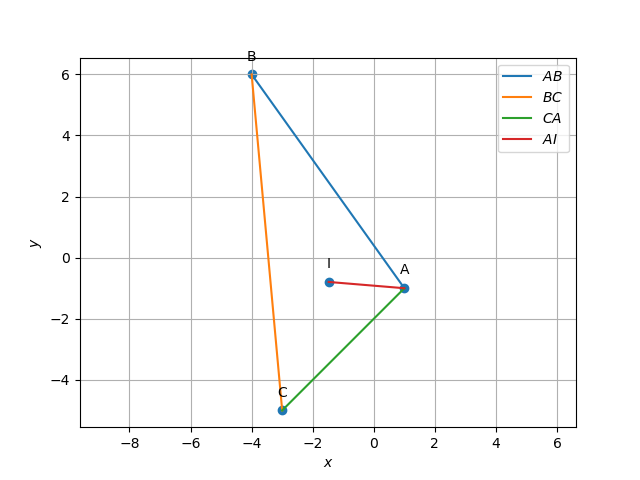
\includegraphics[width=\columnwidth]{solutions/1/5/1/figs/angular_bisector.png}
	\caption{Triangle generated using python}
	\label{fig:angular_bisector}
	\end{figure}
	As we can see we will get 2 solutions for $L$. This is because one of them is internal angular bisector and the other is the external angular bisector. Internal angular bisector can be evaluated if we take + in the above formula.
	Hence, $L$ is given by,
	\begin{align}
		\frac{\vec{n}_{3}^{\top} \vec{x}-c_{3}}{\norm{\vec{n}_{3}}}&=\frac{\vec{n}_{2}^{\top} \vec{x}-c_{2}}{\norm{\vec{n}_{2}}}\\
		\implies \brak{\frac{\vec{n_{3}}}{\norm{\vec{n_{3}}}}-\frac{\vec{n_{3}}}{\norm{\vec{n_{3}}}}} \vec{x}&=\brak{\frac{c_{3}}{\norm{\vec{n_{3}}}}-\frac{c_{2}}{\norm{\vec{n_{2}}}}}\\
		\implies \brak{\frac{\myvec{7&5}}{\sqrt{74}}-\frac{\myvec{1&-1}}{\sqrt{2}}} \vec{x}&=\frac{2}{\sqrt{74}}-\frac{2}{\sqrt{2}}\\
		\implies \myvec{\frac{7-\sqrt{37}}{\sqrt{74}}&\frac{5+\sqrt{37}}{\sqrt{74}}}\vec{x}&=\frac{2-2\sqrt{37}}{\sqrt{74}}
	\end{align}
	Hence, the internal angluar bisector of angle $A$, $L$ will be,
	\begin{align}
		\implies\myvec{\frac{7-\sqrt{37}}{\sqrt{74}}&\frac{5+\sqrt{37}}{\sqrt{74}}} \vec{x}=\frac{2-2\sqrt{37}}{\sqrt{74}}
		\label{eq:1.5.1}
	\end{align}
	
